
       
\section{Programação por Restrições}
%%%%%%%%%%%%%%%%%%%%%%%%%%
\begin{frame}
\frametitle{Programação por Restrições}
\label{incio_PR}
\begin{minipage}{0.47\textwidth}
    \begin{itemize}
        \item Conceituar a PR
        \item Princípios
        \item \textcolor{magenta}{\textbf{03 exemplos $\Rightarrow$ \ref{3_exemplos}}}
        \item 03 técnicas 
        \item Aprendizagem da PR via estudos de casos
        \item Vamos dividir esta seção (Exemplos: \ref{3_exemplos})
    \end{itemize}
\end{minipage}
\begin{minipage}{0.5\textwidth}
\begin{figure}[ht!]
\begin{center}

\includegraphics[width=1.2\textwidth, height=0.40\textheight]{figures/logo_picat_alex.jpg}
\end{center}
\end{figure}
\end{minipage}
\end{frame}
%%%%%%%%%%%%%%%%%%%%%%%%%%%%%%%%%%%%%%%%%%%%%%%%%%%%



\begin{frame}[fragile]
%[fragile, allowframebreaks=0.9]

    \frametitle{Programação por Restrições (PR) -- I}

   \begin{block}{}
     \begin{itemize}
     
      \item A \textcolor{magenta}{Programação por Restrições} (PR) é conhecida por \textcolor{magenta}{\textit{Constraint Programming}} 
      ou simplesmente \textbf{CP}

      \pause
      \item Uma poderosa teoria (e técnica)  que  contorna a complexidade de certos problemas
      exponenciais
             
      \pause
      \item A \textbf{\textcolor{magenta}{PR}} encontrava-se inicialmente dentro da IA e PO, mas como várias outras áreas, tornaram-se
      fortes e autônomas. Atualmente uma área de pesquisa bem forte em alguns países.
      
      \pause
      \item Nesta seção, temos 3 exemplos ilustrar conceitos da \textbf{\textcolor{magenta}{PR}}
    \end{itemize}
    
    \end{block}
    
\end{frame}




\begin{frame}[fragile]
%[fragile, allowframebreaks=0.9]

    \frametitle{Programação por Restrições (PR) -- II}

   \begin{block}{}
     \begin{itemize}

      \item \textcolor{magenta}{\textit{Aproximadamente}} o algoritmo da \textbf{\textcolor{magenta}{PR}} é dado:
       \pause       
          \begin{enumerate}

            \item Avaliar algebricamente  os domínios das variáveis com suas restrições

            \item Intercala iterativamente a \textcolor{magenta}{\textsf{propagação de restrições}} com 
                  um \textcolor{magenta}{\textsf{algoritmo de busca}}

            \item A cada variável instanciada, o processo é repetido sobre as demais variáveis, 
            reduzindo progressivamente o espaço de busca

            \item Volte ao passo inicial até que os domínios permaneçam estáticos
            e que as variáveis apresentem instâncias consistentes
              
          \end{enumerate}
       
        \pause
       \item Este núcleo é uma busca por constantes otimizações

        \pause
       \item Uma das virtudes da \textcolor{magenta}{PR}: 
       a legibilidade e clareza de suas soluções, conhecidos
       como \textcolor{magenta}{\textbf{modelos}}
       
    \end{itemize}
    
    \end{block}
    
\end{frame}


\begin{frame}[fragile]
%[fragile, allowframebreaks=0.9]
\frametitle{Programação por Restrições (PR) -- III}

   \begin{block}{}
     \begin{itemize}
    \item Problemas combinatoriais com domínio nos inteiros são bons candidatos a serem
       resolvidos por \textcolor{magenta}{PR}
      
       \pause
       \item Quando temos problemas que precisamos conhecer \textcolor{magenta}{\textbf{todas}} as respostas, 
    não apenas a melhor resposta
    
      \pause
      \item Quando necessitamos de respostas \textcolor{magenta}{\textit{precisas}} e não apenas as aproximadas.
       Há um custo  computacional a ser pago aqui!
      
    \end{itemize}
    \end{block}
    
\end{frame}



\begin{frame}[fragile]
%[fragile, allowframebreaks=0.9]

\frametitle{Metodologia da  Construção de Modelos}

\begin{figure}[ht!]
\begin{center}

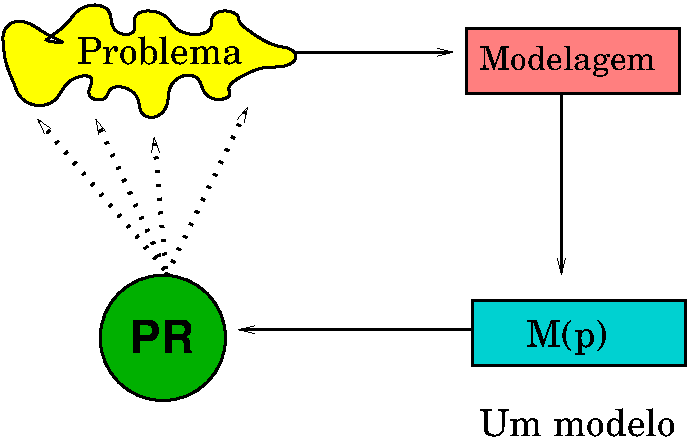
\includegraphics[width=0.70\textwidth, height=0.60\textheight]{figures/problema_modelagem.pdf}

\end{center}
\end{figure}


    
\end{frame}


\begin{frame}[fragile]
%[fragile, allowframebreaks=0.9]

\frametitle{Fluxo de Cálculo da PR}

\begin{figure}[!htb]
\centering
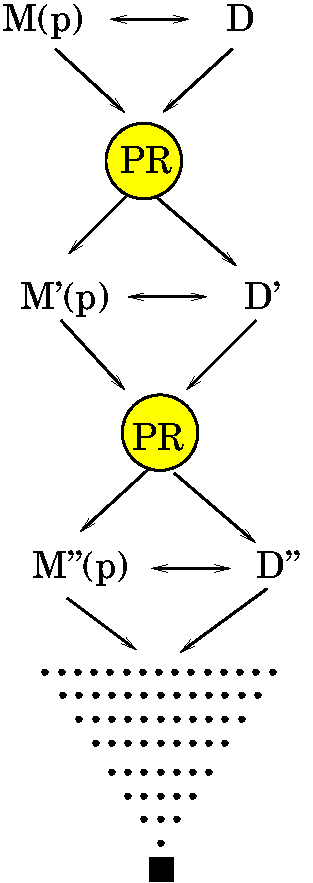
\includegraphics[width=0.30\textwidth, height=0.75\textheight]{figures/dinamica_pr.pdf}
\end{figure}
   
\end{frame}



\begin{frame}[fragile]
%[fragile, allowframebreaks=0.9]

\frametitle{Onde o objetivo da PR é:}

\begin{figure}[!htb]
\begin{center}
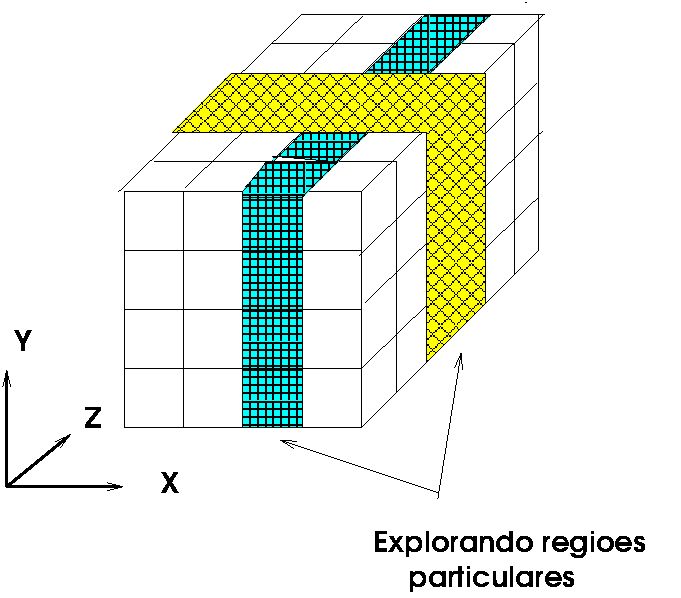
\includegraphics[width=0.70\textwidth, height=0.60\textheight]{figures/reducao_PR_01.pdf}
\caption{Realizar buscas com regiões reduzidas -- promissoras (regiões factíveis de soluções)}
\end{center}
\end{figure}
    
\end{frame}




\begin{frame}[fragile]
%[fragile, allowframebreaks=0.9]

\frametitle{Redução Iterativa em Sub-problemas}

\begin{figure}[!htb]

\begin{center}
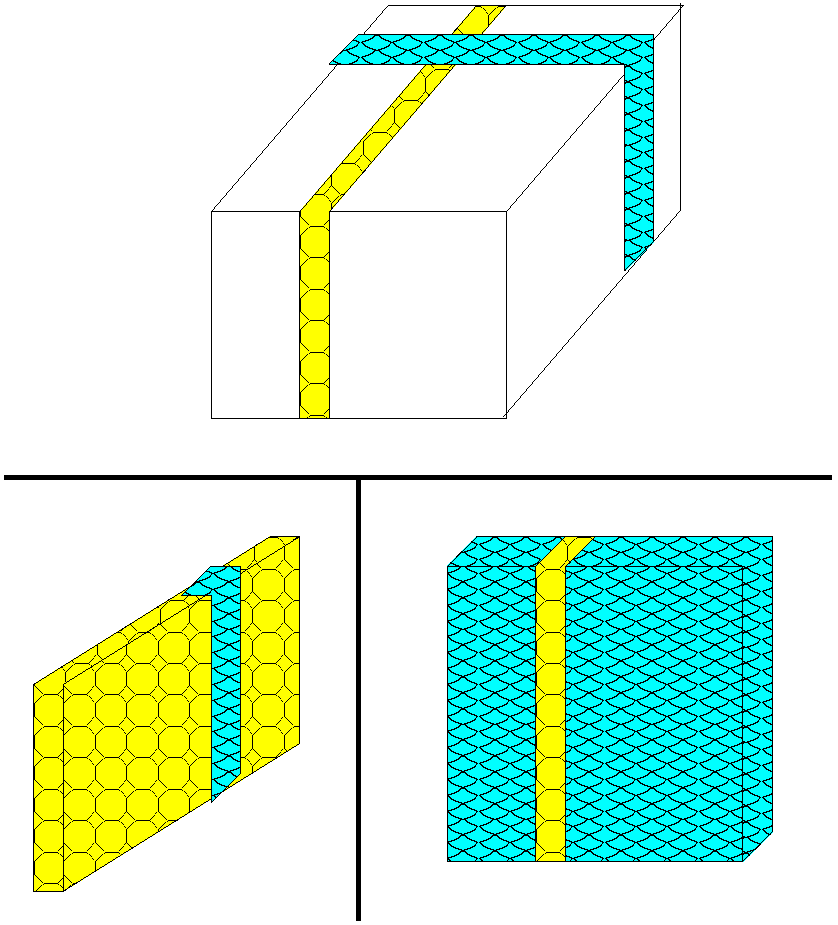
\includegraphics[width=0.70\textwidth, height=0.60\textheight]{figures/reducao_PR_02.pdf}
\caption{Redução de um CP em outros sub-problemas CPs equivalentes}
\end{center}
\end{figure}

    
\end{frame}

%%%%%%%%%%%%%%%%%%%%%%%%%%%%%%%%%%%%%%%%%%%%%%%%%%%%%%%%%%%%%%%%%%%%%%%%%%%%%%%%%%%%

\begin{frame}[fragile]
%[fragile, allowframebreaks=0.9]
\frametitle{Conceitos}

\begin{block}{A PR tem os seguintes elementos:}
    \pause
    \begin{itemize}
    \item Um conjunto de \textbf{variáveis}: $X_1$, $X_2$, $X_3$, ..., $X_n$ 

    \pause
    \item Um conjunto de \textbf{domínios} dessas variáveis: $D_{X_1}$, $D_{X_2}$, $D_{X_3}$, ..., $D_{X_n}$

    \pause
    \item Finalmente, as \textbf{restrições}, que são relações n-árias entre estas variáveis

     \pause
    \item Exemplo: $D_{X_1} = D_{X_2}= \{3,4\}$ e $X_1 \neq X_2$

\end{itemize}

\end{block}
    
\end{frame}

%%%%%%%%%%%%%%%%%%%%%%%%%%%%%%%%%%%%%%%%%%%%%%%%%%%%%%%%%%%%%%%%%%%%%%%%%%%%%%%%%%%%
\begin{frame}[fragile]
%[fragile, allowframebreaks=0.9]
\frametitle{PR e Picat}

\begin{block}{}

\begin{itemize}
    \item Para o exemplo anterior um  código em Picat é dado por:
      \pause
    \begin{itemize}
        \item \texttt{[X1, X2] :: 3..4}
        \item \texttt{X1 \#!= X2} 
     \end{itemize}  
      
      \pause
     \item Em resumo, as relações da PR tem o símbolo `\textbf{\textcolor{magenta}{{\#}}}' 

  \pause
  \item Para tornar toda esta sintaxe da PR disponível, Picat 
        tem um módulo para suporte da PR:\\
         \textcolor{magenta}{\texttt{import cp}}
    
\end{itemize}

\end{block}
    
\end{frame}

%%%%%%%%%%%%%%%%%%%%%%%%%%%%%%%%%%%%%%%%%%%%%%%%%%%%%%%%%%%%%%%
\begin{frame}[fragile] 

\frametitle{Exemplos}

\label{3_exemplos}
\begin{block}{}
\begin{enumerate}
  \item Soma de dois números primos (problema \textit{ad-hoc})
  $\Rightarrow $ \ref{1o_exemplo}
  
  
  \pause
  \item Escala (simplificada) de consultórios médicos (uso de
  matriz)   $\Rightarrow $ \ref{2o_exemplo}
    
  \pause
  \item Caixeiro-viajante (uso de matriz binária de decisão) -- diferente
  da solução do Hakank, aqui discutida $\Rightarrow $ \ref{3o_exemplo}
      
\end{enumerate}
\end{block}

  \begin{center}
\begin{itemize}

    \item   \textbf{\textcolor{magenta}{Basicamente, 3 problemas distintos!}}
    
 \item   \textbf{\textcolor{magenta}{Volte ao início da seção $\Rightarrow$ \ref{incio_PR} }  }

  \end{itemize}  

  \end{center}

\end{frame}

%%%%%%%%%%%%%%%%%%%%%%%%%%%%%%%%%%%%%%%%%%%%%%%%%%%%%%%%%%%%%%%%%%%%%%%%%%%%%%%%%%%%


\begin{frame}[fragile] 
\label{1o_exemplo}
\frametitle{Exemplo -- 01 -- Soma de Números Primos}

\begin{itemize}
  \item Dado um número par qualquer, $N_{PAR}$, encontre  dois de números primos, $N_1$ e $N_2$,
diferentes entre si, que somados deêm este número 
par.

\pause
\item Exemplo:\\
Seja o PAR = 18\\
Uma solução:\\
$N_1 = 7$  e $N_2 = 11$\\
pois\\
$N_1 + N_2 = 18$
\end{itemize}

\end{frame}
%%%%%%%%%%%%%%%%%
\begin{frame}[fragile] 

\frametitle{Modelagem do Problema}

\begin{itemize}
  \item  $N_1$ e $N_2$ assumem valores no domínio dos números primos. \\
  Logo, é importante ter os números primos prontos!

  \pause
   \item A soma destes números é o par fornecido como entrada, $N_{PAR}$:\\
         $N_1 + N_2 = N_{PAR}$

  \pause
  \item  $N_1$ e $N_2$  são diferentes entre si\\
   $N_1 \neq N_2$

  \pause
  \item Como são inteiros: $N_1 < N_{PAR}$ e $N_2 < N_{PAR}$ \\
  Sim, é óbvio, mas isto faz uma redução significativa de domínio!

\end{itemize}

\end{frame}


%%%%%%%%%%%%%%%%%%%%%%%%%%
\begin{frame}[fragile]
 \frametitle{Código Completo}

\begin{itemize}
  \item Acompanhar as explicações do código de:\\
\url{https://github.com/claudiosa/CCS/blob/master/picat/soma_N1_N2_primos_CP.pi}

  \item Confira a execução e testes
\end{itemize}
\end{frame}


%%%%%%%%%%%%%%%%%%%%%%%%%%
\begin{frame}[fragile] 

\frametitle{Código em Partes}

\begin{footnotesize}
\begin{verbatim}
modelo => 
    PAR = 382,
    Variaveis = [N1,N2],
    % Gerando um domino soh de primos
    % L_dom = [I : I in 1..1000, eh_primo(I) == true],   %OU
    L_dom = [I : I in 1..1000, prime(I)],
    Variaveis :: L_dom,
\end{verbatim}
\end{footnotesize}
   
   
   
   \begin{itemize}
   \pause
     \item Uma ótima estratégia: sair com um \textbf{\textcolor{magenta}{domínio de números candidatos}}!
   \pause
     \item O par da entrada: \textcolor{magenta}{\textbf{382}}

     \item Quanto maior este valor, maior o número de soluções?
   \end{itemize}

    
\end{frame}
%%%%%%%%%%%%%%%%%
\begin{frame}[fragile] 

\frametitle{Código em Partes}

\begin{footnotesize}
\begin{verbatim}
    % RESTRICOES
    N1 #!= N2,
    N1 #< PAR,  
    N2 #< PAR,
    N1 + N2 #= PAR,
  
	% A BUSCA
	solve([ff], Variaveis),
  % UMA SAIDA
	printf("\n  N1: %d\t N2: %d", N1,N2),
	printf("\n.....................................")
	.
\end{verbatim}
\end{footnotesize}
    
\end{frame}
%%%%%%%%%%%%%%%%%
\begin{frame}[fragile] 

\frametitle{Código em Partes}

\begin{footnotesize}
\begin{verbatim}
import cp.

% main => modelo	.
% main ?=> modelo, fail.	
% main =>  true.	

main =>
    L = findall(_, $modelo),
    writef("\n Total de solucoes:  %d \n", length(L)) .

\end{verbatim}
\end{footnotesize}
    
\end{frame}


\begin{frame}[fragile]
%[fragile, allowframebreaks=0.9]

\frametitle{Saída -- I}

\begin{footnotesize}
\begin{verbatim}
Picat> cl('soma_N1_N2_primos_CP').
Compiling:: soma_N1_N2_primos_CP.pi
** Warning  : redefine_preimported_symbol(math): prime / 1
soma_N1_N2_primos_CP.pi compiled in 7 milliseconds
loading...

yes

Picat> main.                      

  N1: 3	 N2: 379
.....................................
  N1: 23	 N2: 359
.....................................
  N1: 29	 N2: 353
.....................................
\end{verbatim}
    
\end{footnotesize}
\end{frame}


\begin{frame}[fragile]
%[fragile, allowframebreaks=0.9]

\frametitle{Saída -- II}

\begin{footnotesize}
\begin{verbatim}
 .....................................
  N1: 353	 N2: 29
.....................................
  N1: 359	 N2: 23
.....................................
  N1: 379	 N2: 3
.....................................
 Total de solucoes:  18 

yes

Picat> 
\end{verbatim}
    
\end{footnotesize}
\end{frame}
%%%%%%%%%%%%%%%%%%%%%%%%%%%%%%%%%%%%%%%%%%%%%%%%%%%%%%%%%%%%%%%%%%%%
\begin{frame}[fragile] 

\frametitle{Exemplo -- 02 -- Escala de Consultórios}
\label{2o_exemplo}
\begin{itemize}
\item Seja um Posto Atendimento Médico, um PA, com 4 consultórios e 7 especialidades
  médicas

\pause
\item O problema é distribuir estes médicos nestes 4 consultórios
tal que alguns requisitos sejam atendidos (restrições  satisfeitas)

\pause
\item A abordagem aqui é ingênua e sem muitos critérios
\end{itemize}

\end{frame}
\begin{frame}[fragile] 

\frametitle{Modelagem do Problema}

\begin{itemize}
  \item  Vamos usar uma matriz bi-dimensional para 
  representar o problema. Linhas $\leftrightarrow$ consultórios (1 a 4), e 
  as colunas $\leftrightarrow$ dias da semana (1 a 5)

  \pause
  \item Esta matriz será preenchida com valores/códigos de 1 a 7, de acordo com a especialidade médica.
  
  \pause
  \item Assim o domínio da matriz \texttt{Quadro} ($4 \times 5$) será
  preenchida com um destes códigos.
   
  \pause
  \item Vamos utilizar restrições globais: \textcolor{magenta}{\texttt{member}} e 
  \textcolor{magenta}{\texttt{all\_different}}

  \pause
  \item As restrições globais se aplicam sobre um conjunto de variáveis.

\end{itemize}

\end{frame}


\begin{frame}
  \frametitle{Matriz de Atribuição}

% Please add the following required packages to your document preamble:
% \usepackage[table,xcdraw]{xcolor}
% If you use beamer only pass "xcolor=table" option, i.e. \documentclass[xcolor=table]{beamer}
\begin{table}[]
\begin{tabular}{|c|c|c|c|c|c|}
\hline
{\color[HTML]{00009B} }                                 & {\color[HTML]{CB0000} \textbf{2a.}}                             & {\color[HTML]{CB0000} \textbf{3a.}}        & {\color[HTML]{CB0000} \textbf{4a.}}        & \multicolumn{1}{l|}{{\color[HTML]{CB0000} \textbf{5a.}}}        & \multicolumn{1}{l|}{{\color[HTML]{CB0000} \textbf{6a.}}}        \\ \hline
{\color[HTML]{303498} \textbf{1a. Sala}}                       & {\color[HTML]{009901} \textbf{{[}1..7{]}}}                      & {\color[HTML]{009901} \textbf{{[}1..7{]}}} & {\color[HTML]{009901} \textbf{{[}1..7{]}}} & \multicolumn{1}{l|}{{\color[HTML]{009901} \textbf{{[}1..7{]}}}} & \multicolumn{1}{l|}{{\color[HTML]{009901} \textbf{{[}1..7{]}}}} \\ \hline
{\color[HTML]{303498} \textbf{2a. Sala}}                       & {\color[HTML]{009901} \textbf{{[}1..7{]}}}                      & ...                                        & ...                                        & ...                                                             & ...                                                             \\ \hline
{\color[HTML]{303498} \textbf{3a. Sala}}                       & {\color[HTML]{009901} \textbf{{[}1..7{]}}}                      & ...                                        & ...                                        & ...                                                             & ...                                                             \\ \hline
\multicolumn{1}{|l|}{{\color[HTML]{303498} \textbf{4a. Sala}}} & \multicolumn{1}{l|}{{\color[HTML]{009901} \textbf{{[}1..7{]}}}} & ...                                        & ...                                        & ...                                                             & ...                                                             \\ \hline
\end{tabular}
\end{table}

O domínio de valores: \texttt{1..7} (7 especialidades médicas)

\end{frame}



%%%%%%%%%%%%%%%%%%%%%%%%%%%%%%%%%%%%%%%%%%%%%
\begin{frame}[fragile] 

\frametitle{Modelagem -- Comentários}

\begin{itemize}
  \item A fase de busca e propagação do comando 	\texttt{solve(Critérios, Variáveis)}, 
  há dezenas de combinações possíveis: consultar o guia do usuário
  
  \pause
  \item Tem-se os predicados extras ... são muitos, todos os da CP

  \pause
  \item Finalmente, exemplos sofisticados-- de PR com PICAT:\\
  \url{http://www.hakank.org/picat/} -- \textit{\textbf{My Picat page}} --
  por Hakan Kjellerstrand 

\end{itemize}

\end{frame}

%%%%%%%%%%%%%%%%%%%%%%%%%%
\begin{frame}[fragile]
 \frametitle{Código Completo}

\begin{itemize}
  \item Acompanhar as explicações do código de:\\
\url{https://github.com/claudiosa/CCS/blob/master/picat/horario_medico_CP.pi}

  \item Confira a execução e testes
\end{itemize}
\end{frame}


%%%%%%%%%%%%%%%%%%%%%%%%%%%%%%%%%%%%%%%%%%%%%%%%%%%%
\begin{frame}[fragile] 

\frametitle{Código em Partes}

\begin{footnotesize}
\begin{verbatim}
modelo => 
    Dias = 5, % segunda= 1, ...., sexta-feira = 5
    Consultorio = 4,
    L_dom = [ oftalmo, otorrino, pediatra,  gineco, 
%                1        2          3         4
              cardio, dermato, clin_geral ],
%                5       6        7
   Quadro = new_array(Consultorio, Dias ), %% Lin x Col
   Quadro :: 1 .. L_dom.len , %% operador len . "eh colado"
...
\end{verbatim}
\end{footnotesize}
   
    
\end{frame}
%%%%%%%%%%%%%%%%%%%%%%%%%%%%%%%%%%%%%%%%%%%%%%%%%%%%
\begin{frame}[fragile] 

\frametitle{Código em Partes}

\begin{footnotesize}
\begin{verbatim}
    %% O medico 2 NUNCA trabalha no consultorio 1
    foreach ( J in 1 .. Dias ) 
        Quadro[1,J] #!= 2
    end,
    
    %% O medico 5 NUNCA trabalha no consultorio 4
    foreach ( J in 1 .. Dias ) 
        Quadro[4,J] #!= 5
    end,
...
\end{verbatim}
\end{footnotesize}
    
\end{frame}
%%%%%%%%%%%%%%%%%%%%%%%%%%%%%%%%%%%%%%%%%%%%%%%%%%%%
\begin{frame}[fragile] 

\frametitle{Código em Partes}

\begin{footnotesize}
\begin{verbatim}

  %% O Clin Geral deve vir o maior numero de dias ... 
  %% Esta restricao eh matematicamente é HARD
   foreach ( I in 1 .. Consultorio )
     member(7,[Quadro[I,J] : J in 1..Dias]) 
   end,  
  
  %% Ninguém trabalha no mesmo consultorio em dias seguidos
  foreach ( J in 1 .. Dias )
      all_different( [Quadro[I,J] : I in 1..Consultorio] )
  end,  
 
  %% Ninguém trabalha no mesmo dia em mais de um consultorio
   foreach ( I in 1 .. Consultorio )
      all_different( [Quadro[I,J] : J in 1..Dias] )
   end,  
...  
\end{verbatim}
\end{footnotesize}
    
\end{frame}
%%%%%%%%%%%%%%%%%%%%%%%%%%%%%%%%%%%%%%%%%%%%%%%%%%%%
\begin{frame}[fragile] 

\frametitle{Código em Partes}

\begin{footnotesize}
\begin{verbatim}
	% A BUSCA
	solve([ff], Quadro),
  % UMA SAIDA
	
   printf("\n Uma escolha:"),
   print_matrix( Quadro ),
   print_matrix_NAMES( Quadro , L_dom ),
	 printf(".............................\n") .
\end{verbatim}
\end{footnotesize}
    
\end{frame}
%%%%%%%%%%%%%%%%%%%%%%%%%%%%%%%%%%%%%%%%%%%%%%%%%%%%
\begin{frame}[fragile] 

\frametitle{Código em Partes}

\begin{footnotesize}
\begin{verbatim}
print_matrix_NAMES( M, Lista ) =>
 L = M.length,
 C = M[1].length,
  nl,
   foreach(I in 1  .. L)
     foreach(J in 1  ..  C)
      printf(":%w \t" , print_n_lista( M[I,J], Lista) )
     % printf("(%d,%d): %w " , I, J, M[I,J] ) -- FINE
     end,
     nl
   end.
%%%%%%%%%%%%%%%%%%%%%%%%%%%%%%%%%%%%%%%%%%%%%%%%%%%%%%%%%%%%%%%%%%
print_n_lista( _, [] ) =  [].
print_n_lista( 1, [A|_] ) = A.
print_n_lista( N, [_|B] ) = print_n_lista( (N-1), B ) .
%%%%%%%%%%%%%%%%%%%%%%%%%%%%%%%%%%%%%%%%%%%%%%%%%%%%%%%%%%%%%%%%%%
\end{verbatim}
\end{footnotesize}
    
\end{frame}
%%%%%%%%%%%%%%%%%%%%%%%%%%%%%%%%%%%%%%%%%%%%%%%%%%%%


\begin{frame}[fragile]
%[fragile, allowframebreaks=0.9]

\frametitle{Saída - I}

\begin{footnotesize}
\begin{verbatim}
Picat> cl('horario_medico_CP.pi').
Compiling:: horario_medico_CP.pi
horario_medico_CP.pi compiled in 10 milliseconds
loading...

yes

Picat> main                       

 Uma escolha:
7 1 3 4 5 
4 7 2 3 1 
1 3 7 5 2 
3 2 1 7 4 
\end{verbatim}
  
\end{footnotesize}
\end{frame}

%%%%%%%%%%%%%%%%%%%%%%%%%%%%%%%%%%%%%%%%%%%%%%%%%%%%

\begin{frame}[fragile]
%[fragile, allowframebreaks=0.9]

\frametitle{Saída - II}

\begin{footnotesize}
\begin{verbatim}
:clin_geral 	:oftalmo 	:pediatra 	:gineco 	:cardio 	
:gineco 	:clin_geral 	:otorrino 	:pediatra 	:oftalmo 	
:oftalmo 	:pediatra 	:clin_geral 	:cardio 	:otorrino 	
:pediatra 	:otorrino 	:oftalmo 	:clin_geral 	:gineco 	
....................................
yes
\end{verbatim}
  
\end{footnotesize}
\end{frame}

\begin{frame}[fragile]
%[fragile, allowframebreaks=0.9]

\frametitle{Saída - III}

\begin{footnotesize}
\begin{verbatim}

$ time(picat horario_medico_CP.pi )

 Uma escolha:
7 1 3 4 5 
4 7 2 3 1 
1 3 7 5 2 
3 2 1 7 4 

:clin_geral 	:oftalmo 	:pediatra 	:gineco 	:cardio 	
:gineco 	:clin_geral 	:otorrino 	:pediatra 	:oftalmo 	
:oftalmo 	:pediatra 	:clin_geral 	:cardio 	:otorrino 	
:pediatra 	:otorrino 	:oftalmo 	:clin_geral 	:gineco 	
....................................
real	0m0,023s
user	0m0,007s
sys	0m0,013s
[ccs@gerzat picat]$ 
\end{verbatim}
  
\end{footnotesize}
\end{frame}
%%%%%%%%%%%%%%%%%%%%%%%%%%%%%%%%%%%%%%%%%%%%%%%%%%%%%%%%%%%%%%%%%%%%
\begin{frame}[fragile] 

\label{3o_exemplo}
\frametitle{Exemplo -- 03 -- Caixeiro-Viajante}

\begin{itemize}
\item Este é um exemplo clássico $\Rightarrow $ um NP-Completo $\Rightarrow $ boas soluções
apenas com Colônia de Formigas (técnica da Computação Evolucionária)

\pause
\item Neste exemplo do \textcolor{magenta}{Problema do Caixeiro-Viajante}
 (do inglês: TSP -- \textit{Travelling Salesman Problem}) são discutido com \textcolor{magenta}{\textbf{dois modelos da PR}}, 
 destacando as virtudes de cada um:

\begin{enumerate}
   \item \textcolor{magenta}{\textbf{1o. Modelo}}: usa  restrições globais: \textcolor{magenta}{\texttt{element}} e \textcolor{magenta}{\texttt{circuit}}
  \item  \textcolor{magenta}{\textbf{2o. Modelo}}: usa  variáveis de decisão binária  (uma matriz binária: $N \times N$) 
\end{enumerate}

\pause
\item Tecnicamente, o TSP tem muitas aplicações similares! 
\end{itemize}

\end{frame}

\begin{frame}[fragile]
%[fragile, allowframebreaks=0.9]

\frametitle{O que é o TSP?}

\begin{figure}[!htb]
\begin{center}
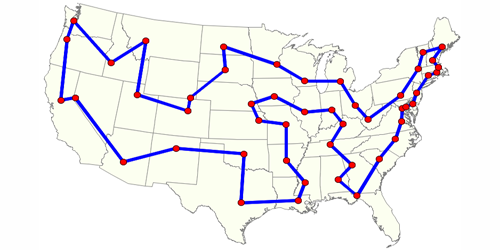
\includegraphics[width=0.80\textwidth, height=0.50\textheight]{figures/tsp01.jpg}
\caption{Passar por algumas cidades uma única vez e retornar a cidade de origem}
\end{center}
\end{figure}
    
\end{frame}



%%%%%%%%%%%%%%%%%%%%%%%%%%%%%%%%%%%%%%%%%%%%%
\begin{frame}[fragile] 

\frametitle{Modelagem -- Comentários}

\begin{itemize}
  \item Usaremos a modelagem matemática de uma \textit{\underline{matriz binária de decisão}}
  
  \pause
  \item Esta abordagem é bem conhecida, porém, eficiente para alguns tipos de problemas

  \pause
  \item Idéia da \textit{\underline{matriz binária de decisão}}: $N$ cidades, logo, há possíveis
  conexões entre elas 
  
%  \pause
%  \item Comentários desta modelagem ao longo do código e detalhes do formalismo matemático
%  em qualquer livro da área de combinatória, PO, e modelagem matemática

\end{itemize}

\end{frame}


%%%%%%%%%%%%%%%%%%%%%%%%%%%%%%%%%%%%%%%%%%%%%%%%%%%%
\begin{frame}[fragile]
\frametitle{Ilustrando -- Matriz de Decisão}


\begin{table}
\centering
\begin{tabular}{|c|c|c|c|c|c|}
\hline 
   & {\color{red} 1}  & {\color{red} 2} & {\color{red}...} &  {\color{red}(N-1)} &  {\color{red} N} \\ \hline
{\color{red}1} & {\color[HTML]{00009B} 0/1} & {\color[HTML]{00009B} 0/1} & ... & {\color[HTML]{00009B} 0/1} & {\color[HTML]{00009B} 0/1} \\ \hline
{\color{red}2} & {\color[HTML]{00009B} 0/1} & ...                        & ...                        & ...  & ...                        \\ \hline
{\color{red}...} & ... & ...                        & ...                        & ... & ...                        \\ \hline
{\color{red}(N-1)} & {\color[HTML]{00009B} 0/1} & ...                        & ...             & ...            & ...                        \\ \hline
{\color{red}N} & {\color[HTML]{00009B} 0/1} & ...                        & ...              & ...           & {\color[HTML]{00009B} 0/1}                        \\ 
\hline 
\end{tabular}

\caption{Matriz de Decisão Binária: $N \times N$}
\end{table}

\begin{itemize}
  \item Uma matriz a ser preenchida com 0's e 1's
  \item Esta matriz pode ter um domínio n-ário 
  \item \textbf{1}: selecionado e \textbf{0}: não-selecionado
\end{itemize}

\end{frame}

%%%%%%%%%%%%%%%%%%%%%%%%%%%%%%%%%%%%%%%%%%%%%%%%%%%%%%%%%%%%%%%%%%
\begin{frame}[fragile]
 \frametitle{Restrições Globais}


  \begin{itemize}
  \item   \textbf{Restrições Globais}: afetam todo modelo ou boa parte deste

   \pause
   \item Algumas conhecidas: \textcolor{magenta}{\texttt{member}} e  \textcolor{magenta}{\texttt{all\_different}}
  
  \pause
  \item Para este modelo, duas novas: \textcolor{magenta}{\texttt{element}} e 
  \textcolor{magenta}{\texttt{circuit}}

  \end{itemize}


\end{frame}

%%%%%%%%%%%%%%%%%%%%%%%%%%
\begin{frame}[fragile]
 \frametitle{Restrição global: \textit{element}}

\begin{verbatim}
element_ex(Vars)  =>  
    X :: 1..4, %% NUM de indices da lista
    element(X , [22, 33, 44, 55], Index),
    Vars = [X , Index],
    solve(Vars).
\end{verbatim}

\end{frame}
%%%%%%%%%%%%%%%%%%%%%%%%%%
\begin{frame}[fragile]
 \frametitle{Restrição global: \textit{element}}

\begin{footnotesize}
\begin{verbatim}
exe04 => 
    Todas_Sol = findall(Uma_Sol , $element_ex(Uma_Sol)),
    foreach( X in Todas_Sol )
      printf("\n Sol %w", X)
    end,
    printf("\n Total de SOL: %d", Todas_Sol.len).  
\end{verbatim}
\end{footnotesize}
\pause

Saída:
\begin{footnotesize}
\begin{verbatim}
 Sol [1,22]
 Sol [2,33]
 Sol [3,44]
 Sol [4,55]
 Total de SOL: 4
\end{verbatim}
\end{footnotesize}
\end{frame}

%%%%%%%%%%%%%%%%%%%%%%%%%%
\begin{frame}[fragile]
 \frametitle{Restrição global: \textit{circuit}}

\begin{verbatim}
circ_ex(L) =>
    L = [X1,X2,X3,X4], 
    L :: 1..4, %% NUM de indices da lista
    circuit(L),
    solve(L).
\end{verbatim}

\end{frame}
%%%%%%%%%%%%%%%%%%%%%%%%%%
\begin{frame}[fragile]
 \frametitle{Restrição global: \textit{circuit}}

\begin{footnotesize}
\begin{verbatim}
exe02 => 
    Todas_Sol = findall( Uma_Sol , $circ_ex(Uma_Sol)),
    foreach( X in Todas_Sol )
      printf("\n Sol %w", X)
    end,
    printf("\n Total de SOL: %d", Todas_Sol.len).  
\end{verbatim}
\end{footnotesize}
\pause

Saída:
\begin{footnotesize}
\begin{verbatim}
 Sol [2,3,4,1]
 Sol [2,4,1,3]
 Sol [3,1,4,2]
 Sol [3,4,2,1]
 Sol [4,1,2,3]
 Sol [4,3,1,2]
 Total de SOL: 6
\end{verbatim}
\end{footnotesize}
\end{frame}


\begin{frame}[fragile]
\frametitle{Código Completo}

\begin{itemize}
\item Acompanhar as explicações do $1^{o.}$ modelo:\\
\url{https://github.com/claudiosa/CCS/blob/master/picat/tsp_ESTUDO_hakan.pi}


\item Acompanhar as explicações do $2^{o.}$ modelo:\\
\url{https://github.com/claudiosa/CCS/blob/master/picat/tsp_CP.pi}

\item Confira a execução e testes
\end{itemize}

\end{frame}

%%%%%%%%%%%%%%%%%%%%%%%%%%%%%%%%%%%%%%%%%%%%%%%%%%%%
\begin{frame}[fragile]
\frametitle{$1^{o.}$ Modelo para o TSP -- Nilsson e Hakan}

\begin{footnotesize}
\begin{verbatim}
% Original formulation from Nilsson cited above.
% Codifificado por HAKAN e CCS
tsp_test(nilsson, Cidades, Custo) =>
   Cidades   = [X1,X2,X3,X4,X5,X6,X7],
   %% a matriz adjacencia - do mapa - 7 cidades
   element(X1,[ 0, 4, 8,10, 7,14,15],C1),
   element(X2,[ 4, 0, 7, 7,10,12, 5],C2),
   element(X3,[ 8, 7, 0, 4, 6, 8,10],C3),
   element(X4,[10, 7, 4, 0, 2, 5, 8],C4),
   element(X5,[ 7,10, 6, 2, 0, 6, 7],C5),
   element(X6,[14,12, 8, 5, 6, 0, 5],C6),
   element(X7,[15, 5,10, 8, 7, 5, 0],C7),
   Custo #= C1+C2+C3+C4+C5+C6+C7 ,
   circuit( Cidades ) ,
   solve([$min(Custo)], Cidades).
\end{verbatim}
\end{footnotesize}

\end{frame}

%%%%%%%%%%%%%%%%%%%%%%%%%%%%%%%%%%%%%%%%%%%%%%%%%%%%
\begin{frame}[fragile]
 \frametitle{Saída}

\begin{footnotesize}
\begin{verbatim}
$ picat tsp_ESTUDO_hakan.pi 
Cidades: [2,7,1,3,4,5,6]	Custo: 34
 A viagem: 
Da cidade 1 --> 2 custa: 4	 Acumulado: 4
Da cidade 2 --> 7 custa: 5	 Acumulado: 9
Da cidade 7 --> 6 custa: 5	 Acumulado: 14
Da cidade 6 --> 5 custa: 6	 Acumulado: 20
Da cidade 5 --> 4 custa: 2	 Acumulado: 22
Da cidade 4 --> 3 custa: 4	 Acumulado: 26
Da cidade 3 --> 1 custa: 8	 Acumulado: 34
\end{verbatim}
\end{footnotesize}
\pause

\begin{itemize}
  \item \textcolor{red}{A importância deste modelo: facilmente se entende o TSP}
  \pause
   \item \textcolor{red}{Hakan fez uma versão genérica para este modelo, de bom desempenho!}
  \pause
   \item \textcolor{red}{O $2^{o.}$ modelo tem importância como técnica para PR!}


\end{itemize}



\end{frame}
%%%%%%%%%%%%%%%%%%%%%%%%%%%%%%%%%%%%%%%%%%%%%%%%%%%%

\begin{frame}[fragile]
\frametitle{$2^{o.}$ Modelo para o TSP -- Usando Matriz de Decisão}

\begin{footnotesize}
\begin{verbatim}
import cp,util.
matriz_adj(Matrix) =>
   Matrix = 
       [[ 0, 4, 8,10, 7,14,15],
        [ 4, 0, 7, 7,10,12, 5],
        [ 8, 7, 0, 4, 6, 8,10],
        [10, 7, 4, 0, 2, 5, 8],
        [ 7,10, 6, 2, 0, 6, 7],
        [14,12, 8, 5, 6, 0, 5],
        [15, 5,10, 8, 7, 5, 0]].
\end{verbatim}
\end{footnotesize}


\begin{itemize}
  \item Os dados são os mesmos do exemplo anterior
  \item Poderia ser feita leitura via arquivos: ver exemplos de entrada e saída no GitHub
  \item Comentários no código e aúdio
  \end{itemize}

\end{frame}

\begin{frame}[fragile] 

\frametitle{Código em Partes}

\begin{footnotesize}
\begin{verbatim}
tsp_D(Matriz, Cidades, M_Decisao, Custo) =>
   Len = Matriz.length, %% N x N cidades
   Cidades = new_list(Len), %%% 1a. dimensao
   Cidades :: 1..Len,
   % grafo de DECISAO que representa o resultado dos nos escolhidos
   M_Decisao = new_array (Len, Len),
   M_Decisao :: 0..1 ,
\end{verbatim}
\end{footnotesize}
\pause

\begin{footnotesize}
\begin{verbatim}
%  calculate upper and lower bounds of the Costs list -- HAKAN
   % repensar MELHORAR .....
   SOMA_Dists = sum([Matriz[I,J] : I in 1..Len, 
                J in 1..Len, Matriz[I,J] > 0]),
   MinDist = 0,
   MaxDist = SOMA_Dists,
   Custo :: 0..MaxDist,
\end{verbatim}
\end{footnotesize}    
    
\end{frame}


\begin{frame}[fragile] 

\frametitle{Código em Partes}

\begin{footnotesize}
\begin{verbatim}
% Se NAO HOUVER CONEXAO ou  ARCO = 0 entao não há conexão
  foreach(I in 1..Len , J  in 1..Len)
    (Matriz[I,J] #= 0) #=> (M_Decisao[I,J] #= 0)
  end,    
\end{verbatim}
\end{footnotesize}
\pause

\begin{footnotesize}
\begin{verbatim}
% Para todas linhas, a soma das colunas é igual a 1
% UMA: uma saida como caminho a ser traçado e somente UMA
  foreach(I in 1..Len)
    sum([M_Decisao[I,J] : J in 1..Len, I != J]) #= 1
  end,     
\end{verbatim}
\end{footnotesize}

\pause

\begin{footnotesize}
\begin{verbatim}
% Para todas colunas, a soma das linhas é igual a 1  
% UMA: uma chegada ao nó de destino e somente UMA chegada
  foreach(J in 1..Len)
   sum([M_Decisao[I,J] : I in 1..Len, I != J]) #= 1
  end,     
\end{verbatim}
\end{footnotesize}    
    
\end{frame}

\begin{frame}[fragile] 
\frametitle{Código em Partes}
\begin{footnotesize}
\begin{verbatim}
%% Relacionar as escolhas da M_Decisao com a
%%  ... sequencia das Cidades. 
  foreach(I in 1..Len , J  in 1..Len)
    ( M_Decisao[I,J] #= 1 ) #<=> ( Cidades[I] #= J )
  end,    
 
  %% garante o circuito entre os nós selecionados
  circuit(Cidades),
 \end{verbatim}
\end{footnotesize}
\pause

\begin{footnotesize}
\begin{verbatim}
%% Função custo a ser minimizada
 Custo #= sum([M_Decisao[I,J] * Matriz[I,J] : 
             I in 1..Len , J  in 1..Len]),

 %% Vars para BUSCA
 Vars = [Cidades, M_Decisao], %% OU  Cidades ++ M_Decisao
 solve([$min(Custo)], Vars ).
\end{verbatim}
\end{footnotesize}    
    
\end{frame}



\begin{frame}[fragile]
 \frametitle{Saída}

\begin{footnotesize}
\begin{verbatim}
$ picat tsp_CP.pi 
M_Decisao: {{0,1,0,0,0,0,0},{0,0,0,0,0,0,1},{1,0,0,0,0,0,0},{0,0,1,0,0,0,0},{0,0,0,1,0,0,0},{0,0,0,0,1,0,0},{0,0,0,0,0,1,0}}
DESTINOS:
      1 2 3 4 5 6 7 
 1 -> 0 1 0 0 0 0 0 
 2 -> 0 0 0 0 0 0 1 
 3 -> 1 0 0 0 0 0 0 
 4 -> 0 0 1 0 0 0 0 
 5 -> 0 0 0 1 0 0 0 
 6 -> 0 0 0 0 1 0 0 
 7 -> 0 0 0 0 0 1 0 
Sequência das Cidades: [2,7,1,3,4,5,6]
Custo: 34

 A viagem: 
Da cidade 1 --> 2 custa: 4	 Acumulado: 4
..........................................
Da cidade 3 --> 1 custa: 8	 Acumulado: 34
\end{verbatim}
\end{footnotesize}

\textcolor{red}{As funções/regras de saída não
foram apresentadas!}

\end{frame}
%%%%%%%%%%%%%%%%%%%%%%%%%%%%%%%%%%%%%%%%%%%%%%%%%%%%





%%%%%%%%%%%%%%%%%%%%%%%%%%%%%%%%%%%%%%%%%%%%%%%%%%%%

\begin{frame}[fragile]
\frametitle{Resumindo a PR}

\begin{itemize}
  \item Há outros métodos para se resolver estes problemas.\\
  Exemplo: Programação Linear, Buscas Heurísticas, AGs, Busca Gulosa  etc

  \pause  
  \item As \textcolor{magenta}{restrições globais} se aplicam sobre um conjunto de variáveis
  e há muitas outras importantes disponíveis no Picat

  \pause
  \item A área é extensa e \textcolor{magenta}{Picat adere há todos requisitos da PR}

  \pause
  \item Resumo da PR: segue por uma notação/manipulação algébrica restrita,
        simplificar e bissecionar as restrições, instanciar variáveis, 
        verificar inconsistências,   avançar sobre as demais variáveis, até que todas 
        estejam instanciadas.
  
  \pause
  \item Enfim, agora é o momento de praticar e aprimorar os conhecimentos $\Rightarrow$ Bons códigos!

\end{itemize}
\end{frame}
